\documentclass[../main.tex]{subfiles}
\graphicspath{{\subfix{../images/}}}
\begin{document}


\section{Exact trig values}
To calculate the exact trig value, we can use a combination of the ratio triangles and compound angle rules.

The ratio triangles are provided in the formula sheet:

\begin{figure}[h]
    \centering
    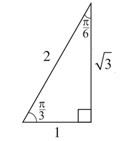
\includegraphics{images/ratiotriangle1.png}
    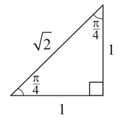
\includegraphics{images/ratiotriangle2.png}
\end{figure}

The compound angle rules are:

\[\sin{(A\pm B)}=\sin{A}\cos{B}\pm \cos{A}\sin{B}\]
\[\cos{(A\pm B)}=\cos{A}\cos{B}\mp \sin{A}\sin{B}\]
\[\tan{A\pm B}=\frac{\tan{A}\pm \tan{B}}{1 \mp \tan{A}\tan{B}}\]

For example, calculate the exact value of $\sin{\Bigl(\frac{\pi}{12}\Bigr)}$

Consider that $\frac{\pi}{12}=\frac{\pi}{3}-\frac{\pi}{4}$

$\sin{(\frac{\pi}{3}-\frac{\pi}{4})}=\sin{\frac{\pi}{3}}\cos{\frac{\pi}{4}}-\cos{\frac{\pi}{3}}\sin{\frac{\pi}{4}}$

From the ratio triangles, we can work out the exact values of each part:

$\sin{\Bigl(\frac{\pi}{12}\Bigr)}=\sin{(\frac{\pi}{3}-\sin{\frac{\pi}{4}})}=\frac{\sqrt{3}}{2}\times \frac{1}{\sqrt{2}}-\frac{1}{2}\times \frac{1}{\sqrt{2}}$

$\sin{\Bigl(\frac{\pi}{12}\Bigr)}=\frac{\sqrt{3}-1}{2\sqrt{2}}$

Rationalising by multiplying by $\frac{\sqrt{2}}{\sqrt{2}}$:

$\sin{\Bigl(\frac{\pi}{12}\Bigr)}=\frac{\sqrt{6}-\sqrt{2}}{4}$
\pagebreak
\subsection*{Harder: using algebra and trig identities}
For angles that where we can't simply use the ratio triangles, we can calculate exact values by forming a quadratic. When the angle we are finding is a factor of 90 or 180, we can rewrite the equation to be sine or cosine of $n\theta$, where $n\theta$ multiplies to 90 or 180.

This then enables us to rearrange using identities and simplify by evaluating sine or cosine of 90 or 180 (or $\pi$ or $2\pi$).

For example, find the exact value of $\sin{18}$.

Since 18 is a factor of 90, we can rewrite this as below. (Note that while it is also a factor of 180, we use the lower value as that requires less working):

$5\theta=90$

$2\theta +3\theta=90$

$2\theta = 90-3\theta$

$\sin{(2\theta)}=\sin{(90-3\theta)}$

$2\sin{\theta}\cos{\theta}=\sin{90}\cos{3\theta}-\cos{90}\sin{3\theta}$

Evaluating $\sin{(90)}=1$ and $\cos{(90)}=0$, we get:

$2\sin{\theta}\cos{\theta}=\cos{3\theta}$

Splitting the $3\theta$ into a sum:

$2\sin{\theta}\cos{\theta}=\cos{(2\theta + \theta)}$

$2\sin{\theta}\cos{\theta}=\cos{2\theta}\cos{\theta}-\sin{2\theta}\sin{\theta}$

Using identities to change the equation so each term has a common factor of $\cos{\theta}$:

$2\sin{\theta}\cos{\theta}=(1-2\sin^2{\theta})\cos{\theta}-2\sin^2{\theta}\cos{\theta}$

Divide through by $\cos{\theta}$

$2\sin{\theta}=(1-2\sin^2{\theta})-2\sin^2{\theta}$

$2\sin{\theta}=1-4\sin^2{\theta}$

Turn into a quadratic and solve using the quadratic equation:

$4\sin^2{\theta}+2\sin{\theta}-1=0$

$\sin{\theta}=\frac{-2\pm \sqrt{20}}{8}=\frac{-2\pm 2\sqrt{5}}{8}=\frac{-1\pm \sqrt{5}}{4}$

Since we know $\sin{18}$ is positive (from out knowledge of the graph), $\sin{18}=\frac{-1+\sqrt{5}}{4}$

\pagebreak
\hypertarget{exacttriglink}{\subsection*{Questions}}
\hyperlink{exacttriganswers}{(Answers - page {\pageref*{Exact trig values answers}})}


\label{Exact trig values}

\begin{enumerate}
    \item $\cos{45}$

    \item $\sin{105}$
    
    \item $\tan{60}$
    
    \item $\cos{\frac{7\pi}{12}}$
    
    \item $\cos{\frac{\pi}{12}}$
    
    \item $\tan{\frac{2\pi}{3}}$
    
    \item $\cos{\frac{5\pi}{12}}$
    
    \item $\sin{\frac{4\pi}{3}}$
    
    \item $\sin{\frac{7\pi}{4}}$
    
    \item $\tan{\frac{3\pi}{4}}$

\end{enumerate}
Using algebra and compound angle rules, find the exact values of the following:
\begin{enumerate}
    \setcounter{enumi}{10}
    \item $\cos{18}$
    
    \item $\sin{36}$
    
    \item $\sin{\frac{2\pi}{5}}$
    
\end{enumerate}





\end{document}